\documentclass[a0,final]{a0poster}
%%%Load packages
\usepackage{multicol} 			%3-column layout
\usepackage[left=2cm,right=2cm,bottom=0cm,top=0cm]{geometry}			%Reset margins
\usepackage{mathpazo}			%Load palatino font & pazo math
\usepackage{color}				%Needed for colour boxes & coloured text
\usepackage{graphics}
\usepackage[export]{adjustbox}
\usepackage{url}
\usepackage{mathtools}
\usepackage{amsmath}
\usepackage{amsfonts}
\usepackage{amssymb}
\usepackage{graphicx}
\usepackage{float}
\usepackage{booktabs}
%\usepackage{dblfnote}

%%%Define colours and lengths
\definecolor{headingcol}{rgb}{1,1,1}			%Colour of main title
\definecolor{boxcol}{rgb}{0.7,0.3,0.2}		%Edge-colour of box and top banner
\fboxsep=1cm							%Padding between box and text
\setlength{\columnsep}{2cm}				%Set spacing between columns
\renewcommand{\familydefault}{\sfdefault}	%Set main text to sans-serif

%%%Format title
\makeatletter							%Needed to include code in main file
\renewcommand\@maketitle{%
\null									%Sets position marker
{
\color{headingcol}\sffamily\VERYHuge		%Set title font and colour
\@title \par}%
\vskip 0.6em%
{
\color{white}\sffamily\large				%Set author font and colour
\lineskip .5em%
\begin{tabular}[t]{l}%
\@author
\end{tabular}\par}%
\vskip 1cm
\par
}
\makeatother

\title{Peering Through Broken Windows: \\Predicting 911 Calls}

\author{Aymen Jaffry \& Peter Bull\\
Harvard University - CS281}

\begin{document}


\hspace{-3cm}								%Align with edge of page, not margin
\colorbox{boxcol}{						%Coloured banner across top
%\begin{minipage}{1189mm}					%Minipage for title contents
\begin{minipage}{600mm}
\maketitle
\end{minipage}
\begin{minipage}{575mm}					%Minipage for title contents

\includegraphics[width=1\textwidth,right]{iacs_logo.png}
\end{minipage}}

\vspace{1cm}

\begin{multicols}{3}							%Use 3-column layout
\raggedcolumns							%Don't stretch contents vertically

%%%Column1
\section*{Overview}
The ``broken windows'' theory, first proposed by Wilson and Kelling in 1982,\footnote{James Q. Wilson and George L. Kelling, Broken Windows: The Police and Neighborhood Safety, Atlantic Monthly 29, 38 (Mar 1982)} supposes that repeated minor misdemeanor behaviors in an area foster more serious crimes. Unpoliced panhandling, loitering, graffiti, and disrepair establish a precedent for anti­social behaviors that has two effects: (1) criminals are more likely to target areas that seem unpoliced, and (2) residents are less likely to report crimes because there is not a history of enforcement. Their argument suggests that by policing minor misdemeanors heavily, cities can reduce the number of violent crimes.\\
\begin{figure}[H]
\centering
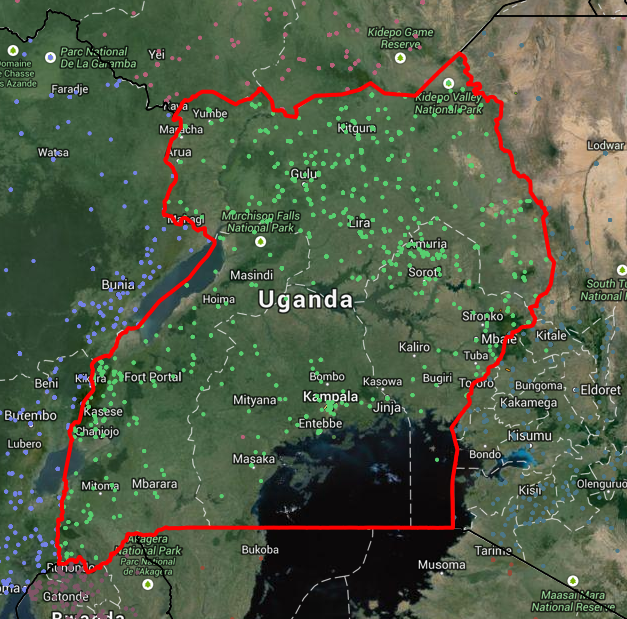
\includegraphics[scale=0.6]{figs/uganda.png}
\caption{Mayor's Hotline Calls about ``broken windows'' in Boston 2011}
\end{figure}
\noindent We put the broken windows theory to the test as a model for a machine learning system that predicts crimes using a set of calls to the ``Mayor's Hotline'' in the Boston area as a proxy for misdemeanors, and a set of calls to 911 as a proxy for crimes. The ``Mayor's Hotline'' calls are for government services and have categories that represent physical neglect and denigration of spaces. Our 911 calls have the location and description of incidents. Using a Poisson-process framework, we build a model for predictive­ policing that uses the broken windows theory to predict where and when crimes will occur that relates 911 calls to the extrinsic covariates in the ``Mayor's Hotline'' data.\\
\begin{figure}[H]
\centering
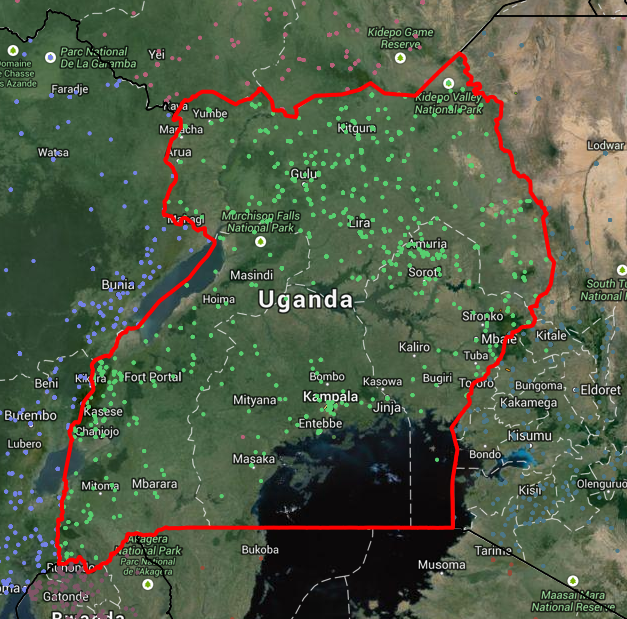
\includegraphics[scale=0.6]{figs/uganda.png}
\caption{911 Calls about Crimes in Boston 2011}
\end{figure}

\columnbreak

\section*{Data}
We have two sets of data which have been provided by the Boston Area Research Initiative.\footnote{http://www.bostonarearesearchinitiative.net/} The ``Mayor's Hotline'' dataset covers calls in 2011 and includes the kind of complaint and the location. We trimmed the dataset down to the following kinds of calls, since they were representative of the ``broken windows'' events in the sociological model: trash, graffiti, and uncivil use. The 911 data we filtered for violent crimes in order to exclude events outside of the scope of our sociological model (such as medical emergencies). We then processed the data into a format where we have a count of broken windows calls and a count of 911 calls for every day of the year for every neighborhood in Boston.\footnote{We had seventeen neighborhoods: Allston-Brighton,} In order to capture the idea that broken windows events are cumulative we added code to compute feature columns that had a cumulative sum for the past $i$ days where $\mathbf{bw}$ is the number of broken windows calls and $t$ is today:
$$ \mathbf{bw}_{t,i} = \sum_{k=1}^i \mathbf{bw}_{t-k}$$
We can adapt our data to test if different time lags, $i$, affect our results. We also added two other feature columns that are temporal covariates: seasonality and day of the week, both of which we could see from observing our data had an affect on the number of 911 calls. Our final data was of the following form:\\
\begin{center}
\begin{tabular}{cccccccc}
Neighborhood & Date & 911 Calls & Season & Day of Week & $\mathbf{bw}_{t}$  & $\hdots$ & $\mathbf{bw}_{t,k}$ \\
\hline
AllstonBrighton & 1/1/2011 & 10 & Winter & Saturday & 10 & $\hdots$ & 25\\
$\vdots$  & $\vdots$  & $\vdots$  & $\vdots$ & $\vdots$ & $\vdots$ & $\vdots$  & $\vdots$ \\
West Roxbury & 12/31/2011 & 4 & Winter & Saturday & 7& $\hdots$ & 21\\
\end{tabular}
\end{center}

\section*{Mathematical Model}
We will be modeling our 911 calls and ``Mayor's Hotline'' calls as point processes in time, where the events in the point-process are denoted $N_{0:t} = \{ 0 < u_1 < \hdots < u_t \}$. Our point process is completely characterized by its conditional intensity function $\lambda(t|\Theta, H(t, x, y))$. By estimating  $\lambda(t|\Theta, H(t, x, y))$, we will be able to predict the number of 911 calls on a given day.\\
\\
To calculate $\lambda(t|\Theta, H(t, x, y))$, we use a Poisson-GLM framework because we are counting events in space and time. We will use $\log \lambda(t|\Theta, H(t, x, y))$ as our natural parameter and define it as follows: \\
\begin{align*}
\log \lambda(t|\Theta, H(t, x, y)) &= \sum_{k=1}^K \theta_k h_k(t,x,y) \\
&\approx \sum_{k=1}^K \theta_k h_k(t) + \sum_{i=1}^I \alpha_i g_i(x,y) \\
\end{align*}
Above we make the assumption that we can separate our covariates that depend on space from those that depend on time. We adapt this method from Truccolo, 2005.\footnote{Matthew R. Fellows John P. Donoghue Emery N. Brown Wilson Truccolo, Uri T. Eden. A point process framework for relating neural spiking activity to spiking history, neural ensemble, and extrinsic covariate effects. Journal of Neurophysiology, (2):1074–1089, 2005.} The first term, $\sum_{k=1}^K \theta_k h_k(t)$, is a weight on our covariates, $\theta_k$ and a history function $h_k(t)$ that takes into account our temporal covariates such as seasonality, week day and 311 calls. Our second term, $\sum_{i=1}^I \alpha_i g_i(x,y)$, has its own weight parameter $\alpha_i$ and a function $g(x,y)$ that represents our spatial covariates. We determine the weights $\{\theta_k\}$ using a Poisson Regression by optimizing the log likelihood. We can then evaluate $\lambda(t|\Theta, H(t, x, y))$ for each day knowing $\{\theta_k\}$ from the Poisson regression and $\{h_k(t,x,y)\}$ as they are our input variables.\\
\\
\noindent Given our general form for $\log \lambda$ we can use the following steps to perform inference:
\begin{enumerate}
\item Use numerical optimization to estimate the MLE weights $\Theta$ and $\{\alpha_i\}$ from our training period $[0,T]$.
\item For a new time $T+\Delta$, we calculate $\{h_k(T+\Delta)\}$ and $g_i(x,y)$ from our data.
\item Calculate our new intensity $\log \lambda(T+\Delta|\Theta, H(T+\Delta, x, y))$ given our weights, $\Theta$ and $\{\alpha_i\}$, and our covariates $\{h_k(T+\Delta)\}$ and $g_i(x,y)$.
\item Using the intensity function, we can calculate $P_n(N|T+\Delta={1,2, ..., J})$ where $J$ is the expected number of 911 calls.
\end{enumerate}

\columnbreak


%%%Column 3
\section*{Results}
\begin{figure}[H]
\centering
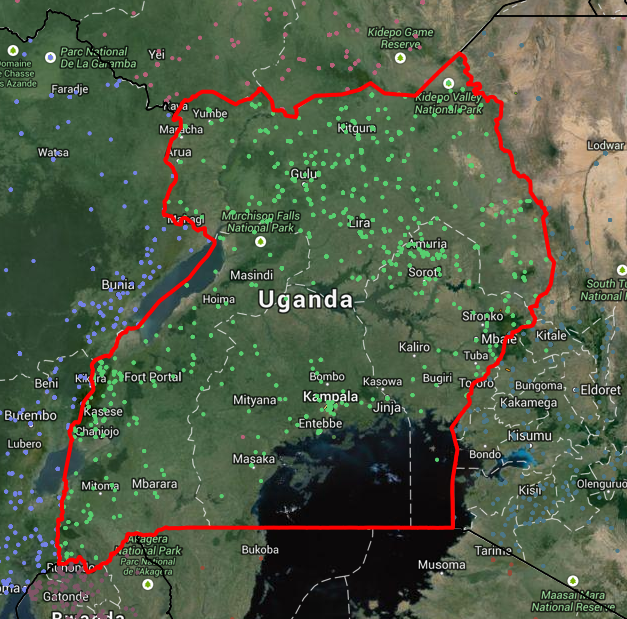
\includegraphics[scale=0.75]{figs/uganda.png}
\caption{Predicted and Actual 911 Calls about Crimes in Boston 2011}
\label{bosgraph}
\end{figure}
As can be seen in Figure \ref{bosgraph}, results for this model do a good job predicting the number of 911 calls on at the geographic resolution of the city of Boston. However, results for the entire city are of limited value. We wanted to see if we can make reliable predictions for finer-grained geographic resolutions: at the level of neighborhoods, census tracts, and census blocks. We have results for all of the neighborhoods in Boston, and have selected three for inclusion in this poster.
\begin{figure}[H]
\centering
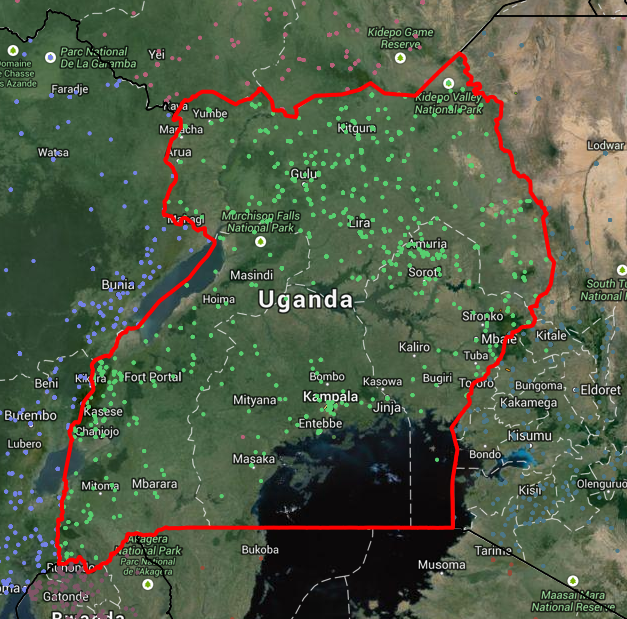
\includegraphics[scale=0.75]{figs/uganda.png}
\caption{Predicted and Actual 911 Calls about Crimes in Boston Neighborhoods 2011}
\label{hoodgraph}
\end{figure}
\noindent The results for our Poisson-GLM give us a set of weights for each feature, and based on these weights we can see how important each feature in our model is. From most to least important, the results for our model are seasonality, ``Mayor's Hotline'' calls the same day, and then the features that represent the cumulative ``Mayor's Hotline'' calls in the past.

\section*{Conclusions}
Given our ordering of features importance, accumulation of ``broken windows'' events does not seem to be the best predictor of crimes. Since ``Mayor's Hotline'' calls the same day has a higher weight than any of the accumulations, we suspect that this feature is a proxy for other confounders that have a different causative story. Of course, our results do not prove or disprove the ``broken windows'' theory, but they do suggest that with the data available it's challenging to build a predictive model using data that's not real-time.\\
\\
In the future, we plan to increase our geographic resolution and see if the results hold for census tracts and census blocks. Ultimately, a system that would be useful need not predict exactly how many crimes will occur in a day. Instead, the system could have a threshold that could indicate when police departments should re-allocate resources to a particular neighborhood.

\section*{Acknowledgements}
We want to thank Professor Ryan Adams, the course staff of CS281 (in particular Scott Linderman), Dan O'Brien at BARI, and Pavlos Protopapas for their help, advice, and support.
\nocite*

%\bibliographystyle{plain}
%\bibliography{halobib}

\end{multicols}
\end{document}
